\chapter{Конструкторский раздел}

\section{Функциональная модель системы}

Функциональная модель системы декомпозиции сложных вопросов представляет процесс преобразования исходного сложного вопроса в набор более простых. Данный процесс реализуется с помощью локальной языковой модели, которая получает специально сформированные инструкции (промпты) для выполнения декомпозиции.

Проектируемая система основана на результатах анализа существующих решений, проведенного в аналитическом разделе. Для реализации выбран подход с использованием локальной языковой модели, что позволяет обеспечить высокую адаптивность к различным типам вопросов при сохранении контекста и логических связей, а также независимость от внешних сервисов.

Для формализации процесса декомпозиции разработана функциональная модель в нотации IDEF0, представленная на диаграммах нулевого и первого уровней (рисунки \ref{fig:constr_idef0_level0}, \ref{fig:constr_idef0_level1}).

\begin{figure}[h]
	\centering
	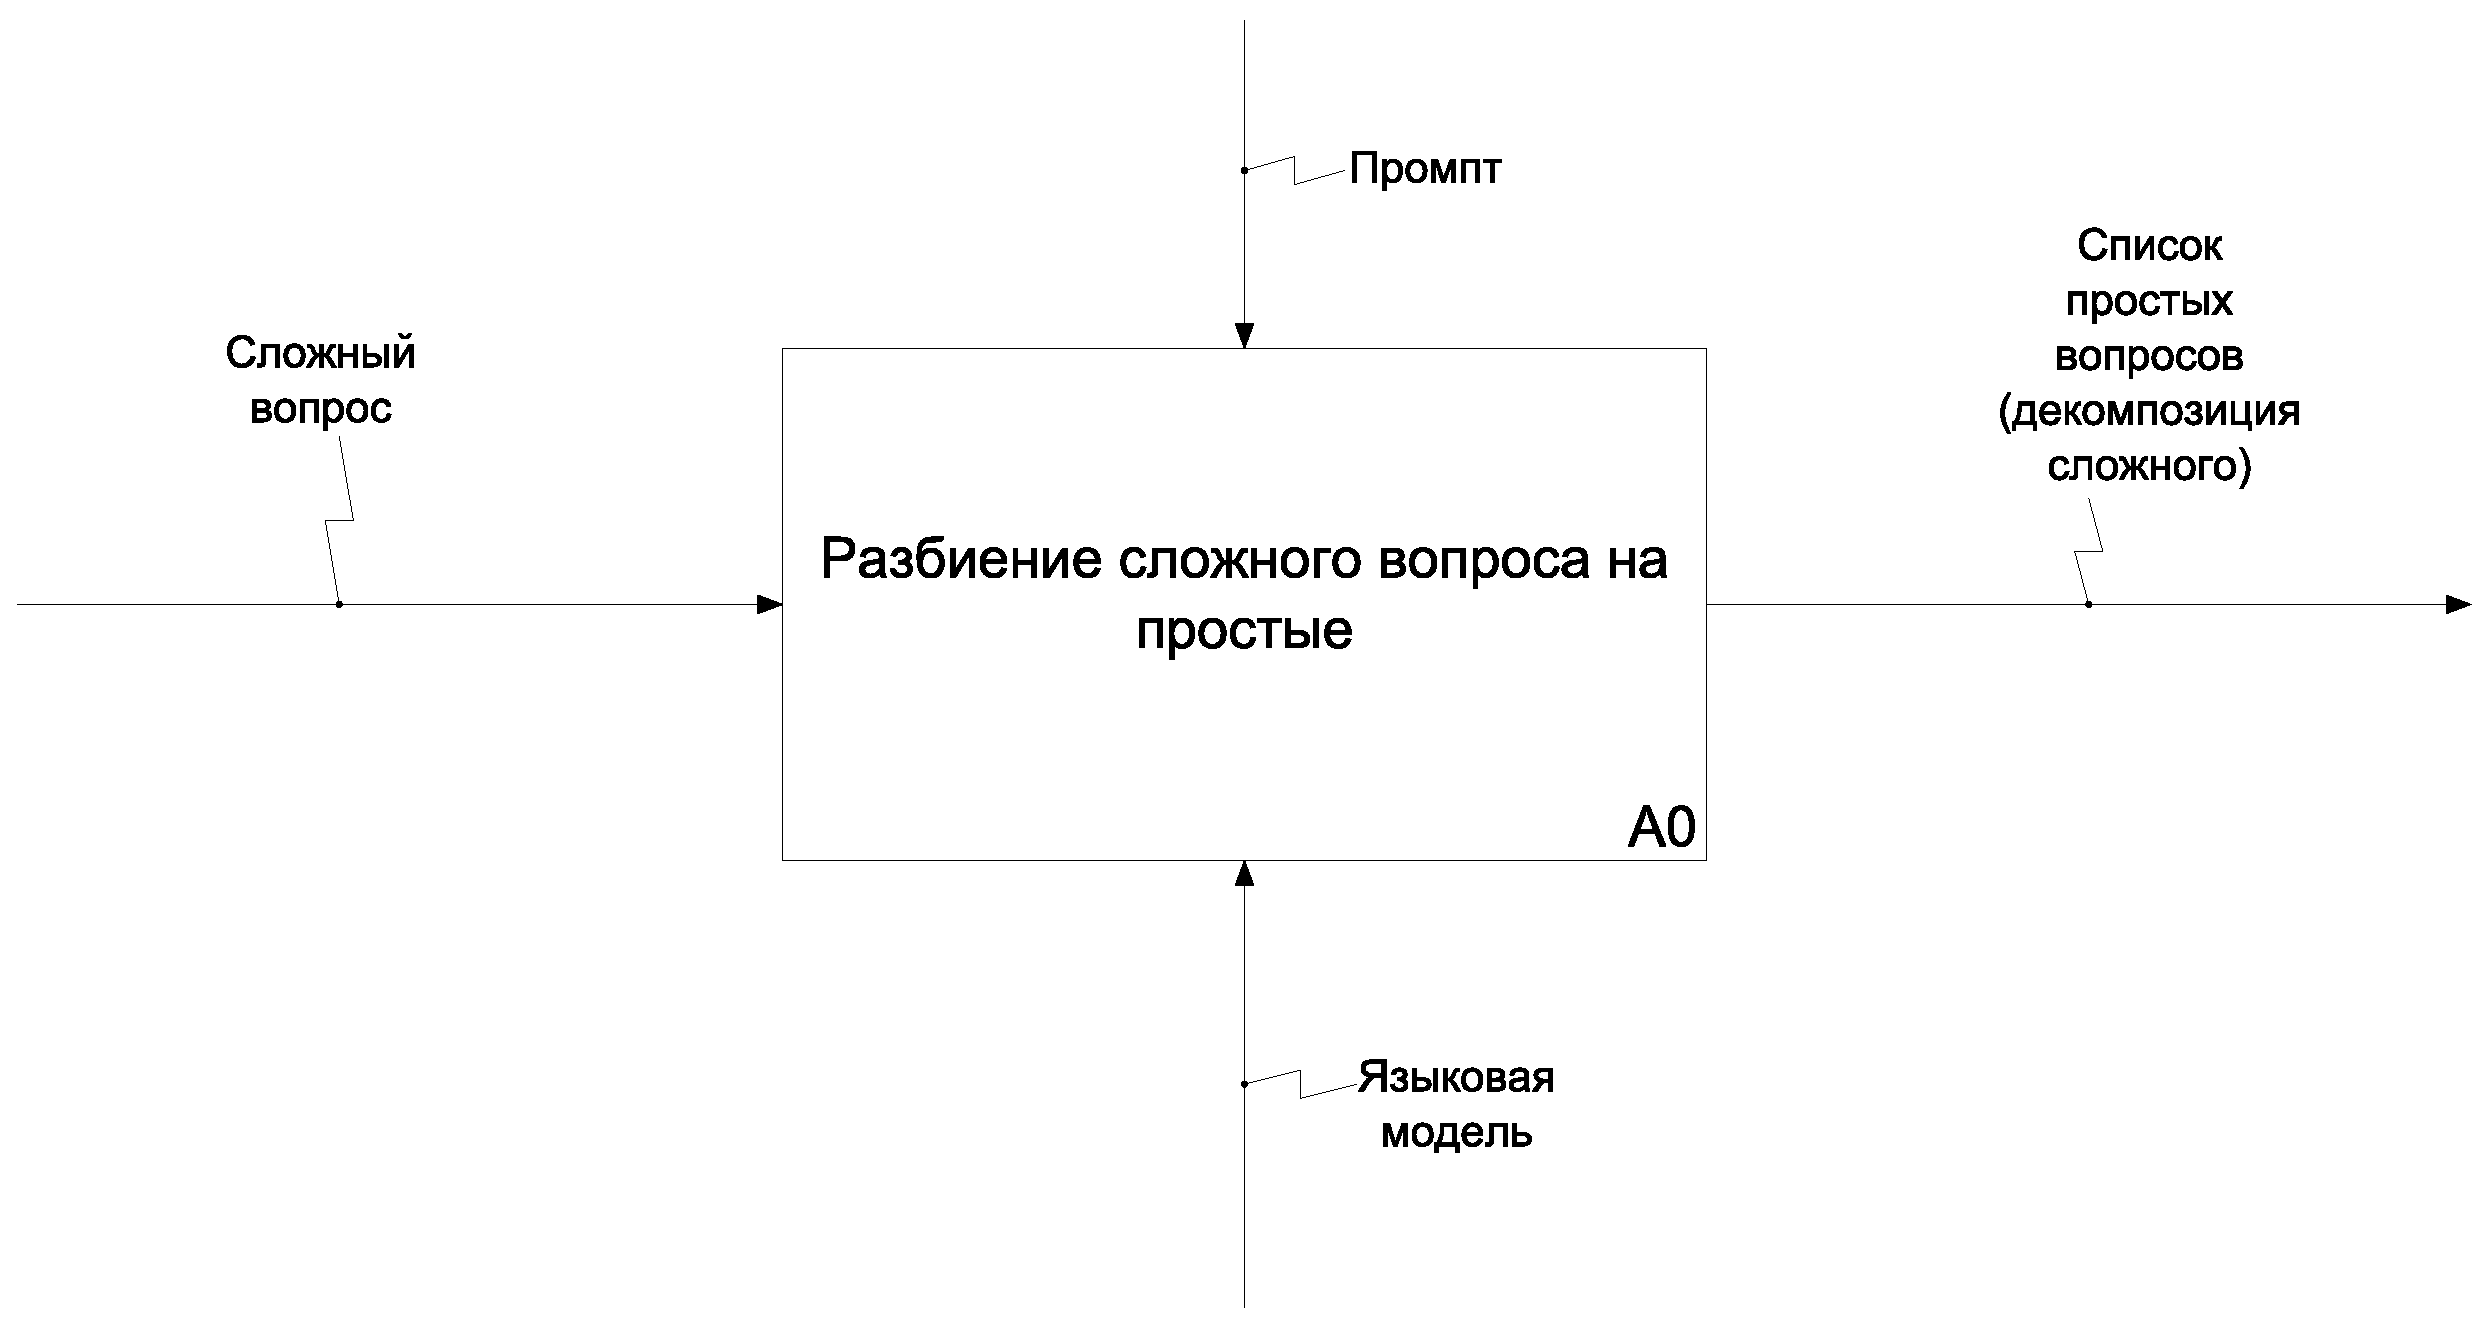
\includegraphics[width=0.8\textwidth]{images/idef0_level0.pdf}
	\caption{Функциональная модель процесса разбиения сложных вопросов (нулевой уровень)}
	\label{fig:constr_idef0_level0}
\end{figure}

\newpage

Для более детального представления структуры системы разработана модель первого уровня, которая включает три последовательных процесса:
\begin{enumerate}
	\item формирование запроса к языковой модели;
	\item взаимодействие с языковой моделью;
	\item формирование результата декомпозиции.
\end{enumerate}

\begin{figure}[h]
	\centering
	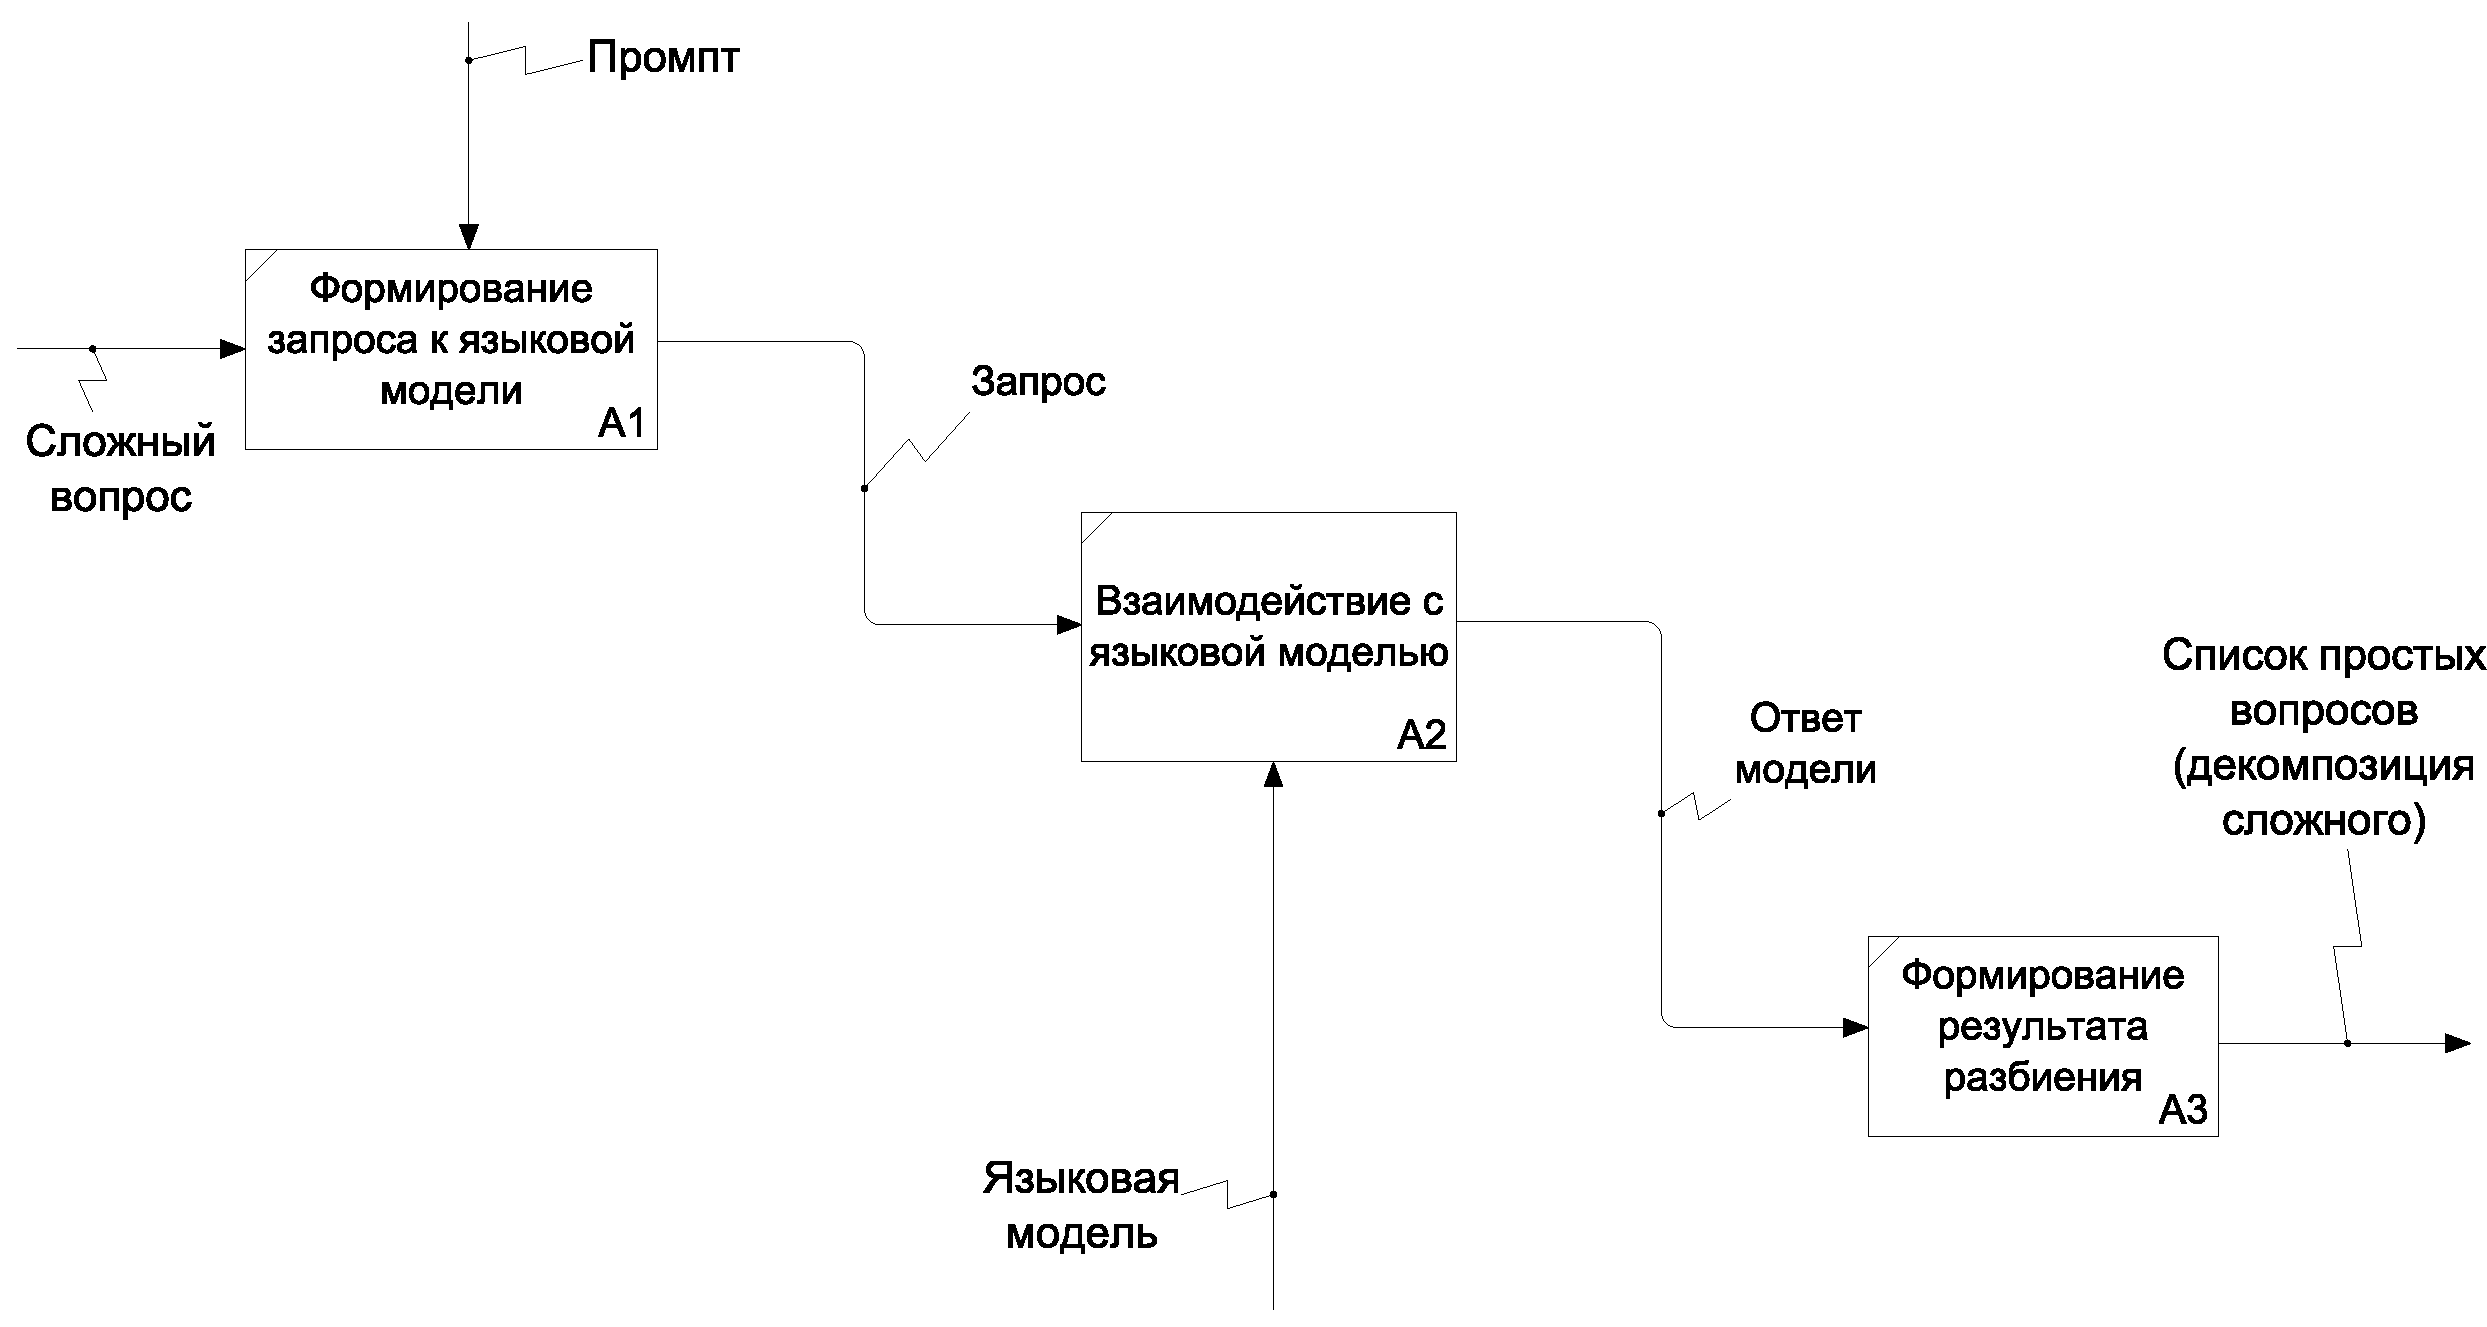
\includegraphics[width=0.8\textwidth]{images/idef0_level1.pdf}
	\caption{Функциональная модель процесса разбиения сложных вопросов (первый уровень)}
	\label{fig:constr_idef0_level1}
\end{figure}

Декомпозиция процесса позволяет выделить три ключевых этапа обработки вопроса. На первом этапе исходный сложный вопрос преобразуется в формат запроса для языковой модели с добавлением промпта. Далее подготовленный запрос передается в языковую модель, которая генерирует ответ согласно полученным инструкциям. На заключительном этапе система обрабатывает полученный от модели ответ, структурирует его и формирует итоговый список простых вопросов.

Разделение на отдельные процессы позволяет локализовать компоненты системы и обеспечить их независимую модификацию и тестирование. Такой подход также упрощает интеграцию различных языковых моделей и форматов представления данных.

\section{Архитектура программного решения}

Программное решение для декомпозиции сложных вопросов построено на модульном принципе, что обеспечивает гибкость системы и возможность ее адаптации к различным требованиям. Архитектура включает три основных модуля, взаимодействующих между собой для обеспечения полного цикла обработки вопросов (рисунок \ref{fig:constr_architecture}).

\begin{figure}[H]
	\centering
	\begin{tikzpicture}[
		box/.style={draw, rectangle, minimum width=6cm, minimum height=1.8cm, thick},
		arrow/.style={->, >=latex, thick},
		node distance=3.5cm
		]
		
		% Модули - располагаем вертикально
		\node[box] (ui) at (0,0) {Модуль консольного интерфейса};
		\node[box] (manager) at (0,-4) {Модуль управления запросами};
		\node[box] (model) at (0,-8) {Модуль взаимодействия с языковой моделью};
		
		% Стрелки вниз по левой части
		\draw[arrow] ([xshift=-1cm]ui.south) -- node[left] {Вопрос} ([xshift=-1cm]manager.north);
		\draw[arrow] ([xshift=-1cm]manager.south) -- node[left] {Запрос} ([xshift=-1cm]model.north);
		
		% Стрелки вверх по правой части
		\draw[arrow] ([xshift=1cm]model.north) -- node[right] {Ответ} ([xshift=1cm]manager.south);
		\draw[arrow] ([xshift=1cm]manager.north) -- node[right] {Результат} ([xshift=1cm]ui.south);
		
	\end{tikzpicture}
	\caption{Архитектура программного решения}
	\label{fig:constr_architecture}
\end{figure}

Основные модули системы и их функции:

\begin{enumerate}
	\item Модуль консольного интерфейса отвечает за взаимодействие с пользователем через командную строку. Основные функции модуля включают чтение сложных вопросов из указанных пользователем текстовых файлов и запись результатов декомпозиции в выходные файлы. Модуль поддерживает базовые команды для управления процессом и настройками приложения.

	\item Модуль управления запросами осуществляет подготовку запроса к языковой модели с добавлением необходимых инструкций и обработку полученных результатов. Данный модуль также выполняет фильтрацию входных запросов и выходных ответов на предмет наличия запрещенных слов по предустановленному списку. Модуль связывает интерфейс пользователя с языковой моделью и обеспечивает корректную передачу данных между ними.

	\item Модуль взаимодействия с языковой моделью обеспечивает коммуникацию с локальной языковой моделью, передачу запросов и получение ответов. Модуль содержит механизмы обработки ошибок для обеспечения надежности системы.
\end{enumerate}

Взаимодействие между модулями построено по принципу последовательной обработки данных. Модуль консольного интерфейса считывает вопрос из указанного пользователем файла и передает его в модуль управления запросами. Этот модуль формирует полный запрос и передает его в модуль взаимодействия с языковой моделью. После получения ответа от модели данные проходят обратный путь: модуль взаимодействия передает их в модуль управления запросами для структурирования, после чего результат передается в модуль консольного интерфейса для записи в выходной файл.

\section{Алгоритмическое обеспечение}



\subsection{Алгоритм формирования запроса к языковой модели}

Алгоритм формирования запроса предназначен для подготовки структурированного запроса к языковой модели, включающего оригинальный вопрос пользователя и специализированный промпт с инструкциями по декомпозиции (рисунок \ref{fig:constr_prompt_algorithm}). Он представляет собой последовательность действий от получения исходного вопроса до формирования полного запроса к модели. 

Алгоритм включает следующие шаги:
\begin{enumerate}
	\item получение исходного вопроса из указанного файла;
	\item загрузка шаблона промпта из конфигурационного файла;
	\item объединение промпта и вопроса пользователя в единый запрос;
	\item проверка запроса на наличие запрещенных слов по предустановленному списку;
	\item форматирование запроса для передачи языковой модели;
	\item возвращение готового запроса для дальнейшей обработки.
\end{enumerate}

Временная сложность алгоритма: $O(n)$, где $n$ -- длина исходного вопроса и промпта.
Требования к памяти: $O(n)$, необходимая память линейно зависит от размера вопроса и промпта.

\begin{figure}[H]
	\centering
	\begin{tikzpicture}[
		start/.style={draw, rounded rectangle, minimum width=4.5cm, minimum height=1cm, thick},
		process/.style={draw, rectangle, minimum width=4.5cm, minimum height=1cm, thick},
		end/.style={draw, rounded rectangle, minimum width=4.5cm, minimum height=1cm, thick},
		arrow/.style={->, >=latex, thick},
		node distance=2cm
		]
		
		% Элементы блок-схемы
		\node[start] (start) {Начало};
		\node[process, below=of start] (input) {Получение вопроса из консоли};
		\node[process, below=of input] (load) {Загрузка шаблона промпта};
		\node[process, below=of load] (combine) {Объединение промпта и вопроса};
		\node[process, below=of combine] (format) {Форматирование запроса};
		\node[end, below=of format] (end) {Конец};
		
		% Стрелки с текстом
		\draw[arrow] (start) -- node[right] {Ввод пользователя} (input);
		\draw[arrow] (input) -- node[right] {Конфигурационный файл} (load);
		\draw[arrow] (load) -- node[right] {Подготовка контекста} (combine);
		\draw[arrow] (combine) -- node[right] {Создание структуры запроса} (format);
		\draw[arrow] (format) -- node[right] {Возврат готового запроса} (end);
		
	\end{tikzpicture}
	\caption{Алгоритм формирования запроса к языковой модели}
	\label{fig:constr_prompt_algorithm}
\end{figure}

\subsection{Алгоритм обработки ответа языковой модели}

Алгоритм обработки ответа предназначен для структурирования результата, полученного от языковой модели, в заданный формат (список вопрос), который ожидает пользователь (рисунок \ref{fig:constr_response_algorithm}).

\begin{figure}[H]
	\centering
	\begin{tikzpicture}[
		start/.style={draw, rounded rectangle, minimum width=4.5cm, minimum height=1cm, thick},
		process/.style={draw, rectangle, minimum width=4.5cm, minimum height=1cm, thick},
		decision/.style={draw, diamond, minimum width=4.5cm, minimum height=2.5cm, aspect=2, thick},
		end/.style={draw, rounded rectangle, minimum width=4.5cm, minimum height=1cm, thick},
		arrow/.style={->, >=latex, thick},
		node distance=2.5cm
		]
		
		% Элементы блок-схемы
		\node[start] (start) {Начало};
		\node[process, below=of start] (receive) {Получение ответа модели};
		\node[decision, below=of receive] (error) {Есть ошибки?};
		\node[process, below=2cm of error, xshift=-4.5cm] (error_handle) {Обработка ошибки};
		\node[process, below=2cm of error, xshift=4.5cm] (parse) {Разбор текста ответа};
		\node[process, below=of parse] (filter) {Фильтрация результатов};
		\node[process, below=of filter] (format) {Форматирование списка};
		\node[end, below=of format] (end) {Конец};
		
		% Стрелки с текстом
		\draw[arrow] (start) -- node[right] {Вопрос от пользователя} (receive);
		\draw[arrow] (receive) -- node[right] {Ответ модели} (error);
		\draw[arrow] (error.west) -- ++(-2.109,0) to[out=-90, in=90] (error_handle.north) node[above, pos=0.5, yshift=2pt] {Да};
		\draw[arrow] (error.east) -- ++(2.109,0) to[out=-90, in=90] (parse.north) node[above, pos=0.5, yshift=2pt] {Нет};
		
		\draw[thick] (error_handle) -- ++(0,-9cm) -| node[left, pos=0.3, yshift=4.8cm] {Сообщение об ошибке} ($(format)!0.5!(end)$);
		\draw[arrow] (parse) -- node[right] {Извлечение вопросов} (filter);
		\draw[arrow] (filter) -- node[right] {Удаление дубликатов} (format);
		\draw[arrow] (format) -- node[right, align=left] {Создание списка \\ простых вопросов} (end);
		
	\end{tikzpicture}
	\caption{Алгоритм обработки ответа языковой модели}
	\label{fig:constr_response_algorithm}
\end{figure}

\newpage

Алгоритм обработки ответа иллюстрирует процесс извлечения и структурирования простых вопросов из текстового ответа языковой модели. Включает проверки на наличие ошибок и корректность формата ответа.

Алгоритм состоит из следующих шагов:
\begin{enumerate}
	\item получение текстового ответа от языковой модели;
	\item проверка на наличие ошибок в ответе модели;
	\item разбор текстового ответа и извлечение отдельных вопросов;
	\item проверка извлеченных вопросов на наличие запрещенных слов;
	\item фильтрация и удаление возможных дубликатов или нерелевантных элементов;
	\item форматирование результата в структурированный список вопросов;
	\item сохранение готового списка простых вопросов в выходной файл.
\end{enumerate}

Временная сложность алгоритма: $O(m)$, где $m$ -- длина ответа языковой модели.
Требования к памяти: $O(m)$, необходимая память линейно зависит от размера ответа.

\section{Сценарий использования системы}

Основной сценарий использования консольного приложения включает:
\begin{enumerate}
	\item запуск приложения через командную строку;
	\item формирование системой запроса к языковой модели;
	\item отправка запроса в локальную языковую модель и получение ответа;
	\item обработка ответа и формирование списка простых вопросов;
	\item запись результата в указанный файл в виде пронумерованного списка простых вопросов.
\end{enumerate}

\section{Требования к консольному интерфейсу}

Консольный интерфейс системы должен обеспечивать:
\begin{itemize}
	\item поддержку пакетного режима обработки нескольких файлов;
	\item поддержку базовых команд: декомпозиция, справка, завершение работы;
	\item отображение процесса обработки запроса (вывод названия текущего процесса);
	\item формирование диагностических сообщений при возникновении ошибок.
\end{itemize}

\section{Процессная модель системы}

Для наглядного представления последовательности операций и взаимодействия между компонентами системы разработана процессная модель декомпозиции сложных вопросов в нотации BPMN (Business Process Model and Notation), представленная на рисунок \ref{fig:constr_bpmn}.

\begin{figure}[H]
	\centering
	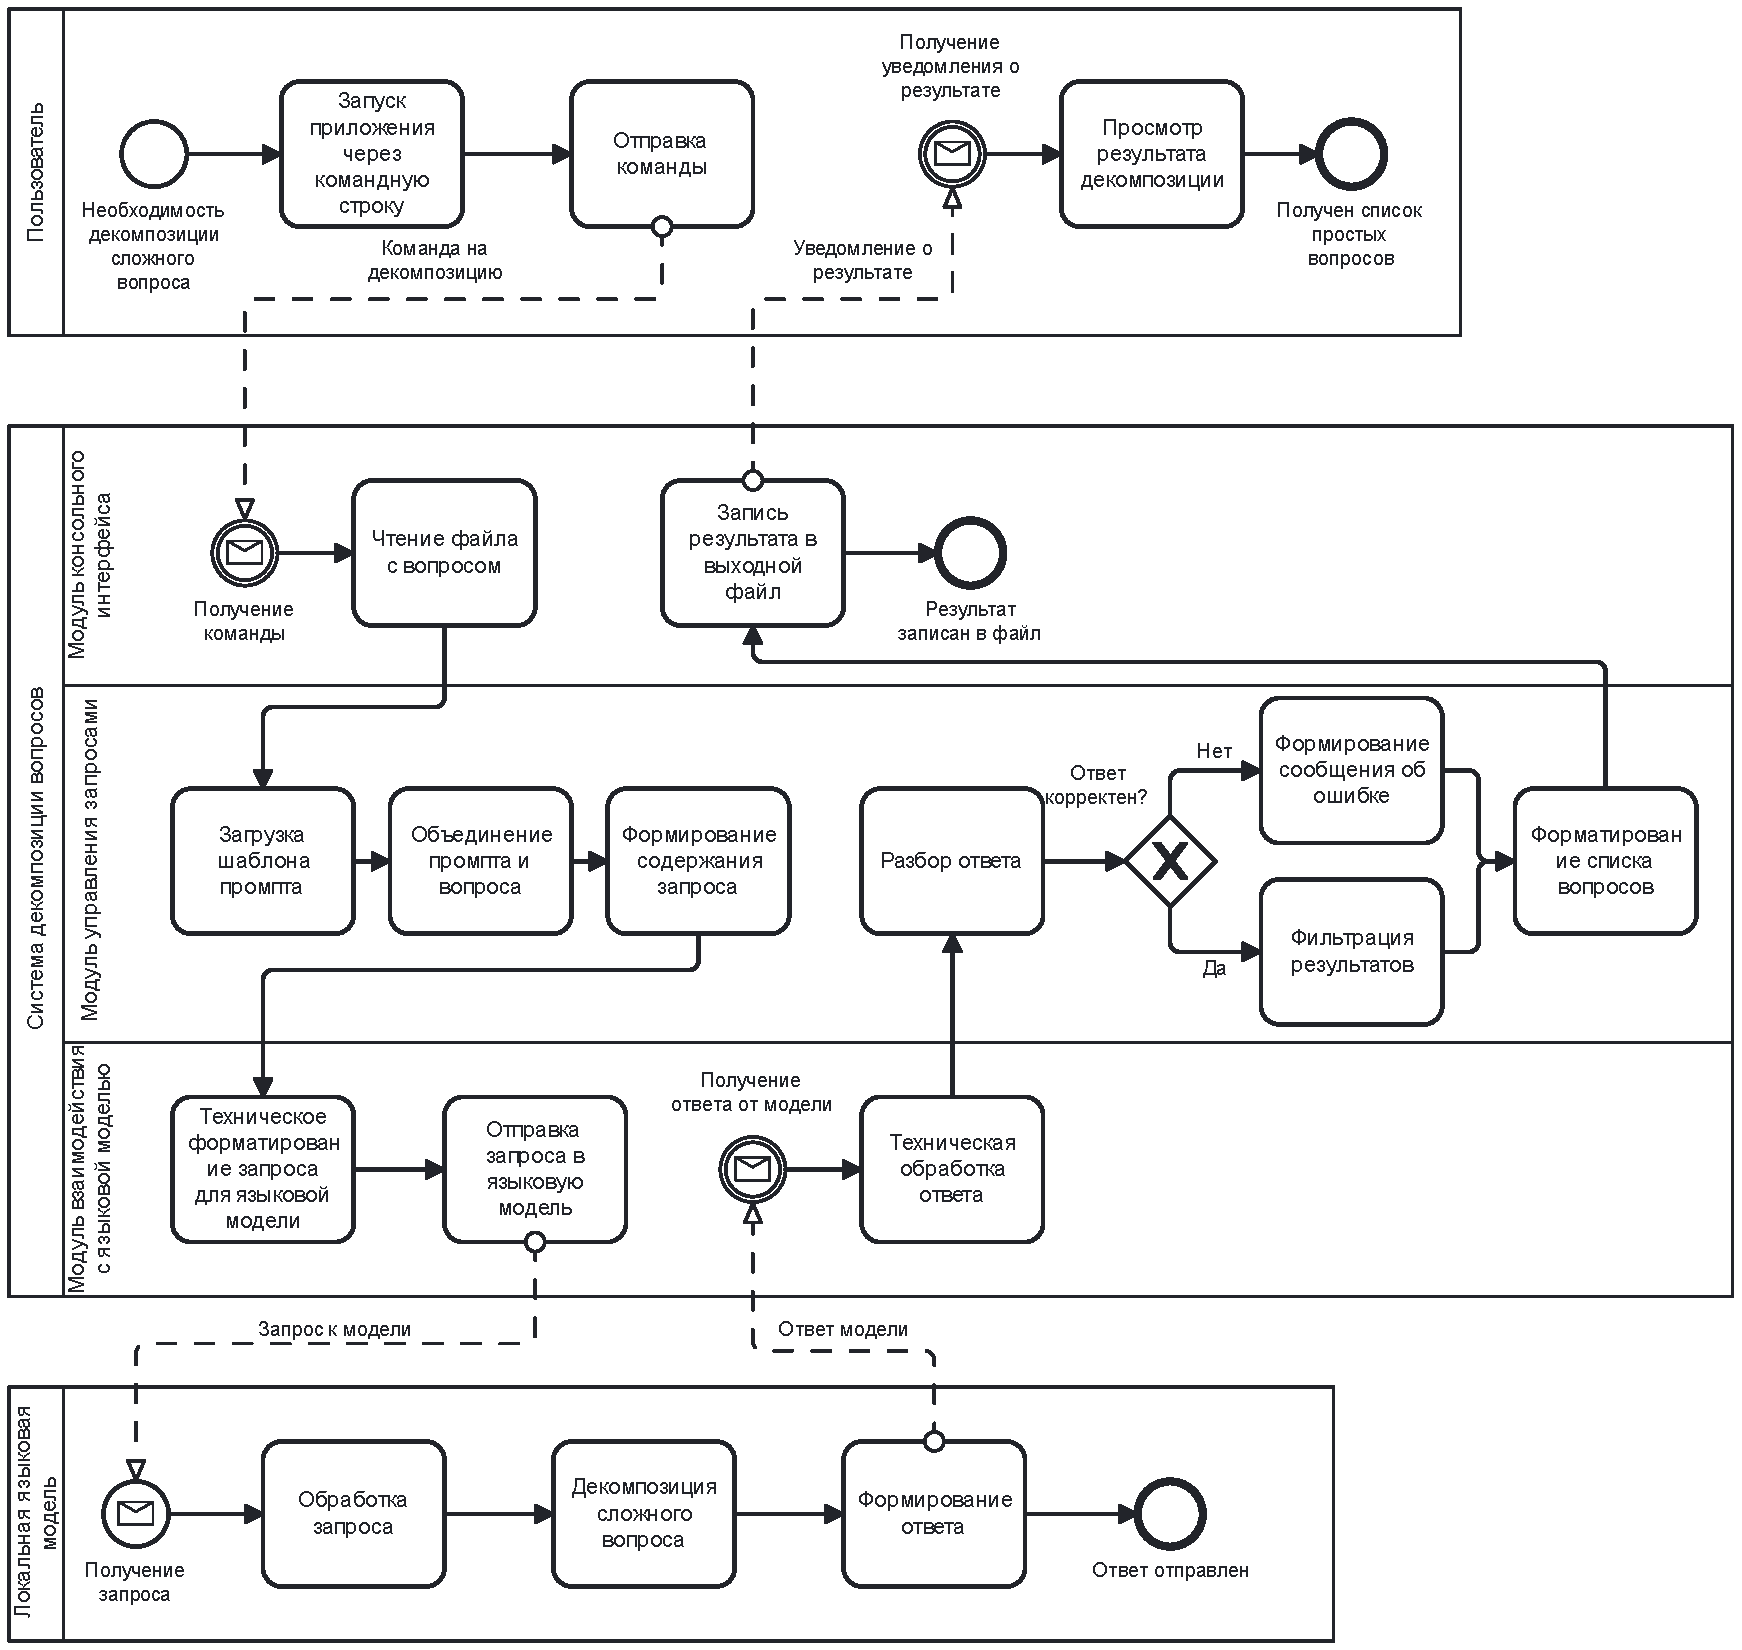
\includegraphics[width=1\textwidth]{images/BPMN.pdf}
	\caption{Процессная модель декомпозиции сложных вопросов в нотации BPMN}
	\label{fig:constr_bpmn}
\end{figure}

Данная модель детализирует взаимодействие четырех основных участников процесса:
\begin{itemize}
	\item пользователь системы, инициирующий декомпозицию вопроса;
	\item модуль консольного интерфейса, обеспечивающий ввод-вывод данных;
	\item система декомпозиции вопросов, включающая модуль управления запросами и модуль взаимодействия с языковой моделью;
	\item локальная языковая модель, выполняющая непосредственную декомпозицию.
\end{itemize}

Представленная процессная модель иллюстрирует полный жизненный цикл декомпозиции вопроса -- от момента запуска приложения пользователем до получения структурированного списка простых вопросов. В модели отражены точки принятия решений, например, проверка корректности ответа модели, которая позволяет обрабатывать нестандартные ситуации.

Модель также демонстрирует распределение задач между тремя основными модулями системы и позволяет визуализировать потоки данных между ними. Такое представление обеспечивает комплексное понимание процесса декомпозиции и возможность анализа системы на предмет оптимизации взаимодействия между компонентами.

\section{Параметры системы}

\subsection{Временные характеристики}

Для обеспечения приемлемого пользовательского опыта система должна соответствовать следующим временным характеристикам:
\begin{itemize}
	\item время формирования запроса к языковой модели: не более 0.01 секунды;
	\item время обработки запроса языковой моделью: не более 60 секунд для сложных вопросов (зависит от размера модели и вычислительных ресурсов);
	\item время обработки ответа и формирования результата: не более 60 секунд (зависит от размера модели и вычислительных ресурсов).
\end{itemize}

\subsection{Параметры языковой модели}

К используемой локальной языковой модели предъявляются следующие требования:
\begin{itemize}
	\item поддержка контекстного окна не менее 2000 токенов для обработки сложных вопросов;
	\item возможность работы с русским языком;
	\item способность следовать инструкциям в промпте для структурированного вывода;
	\item производительность, достаточная для обработки запроса в рамках установленных временных ограничений.
\end{itemize}

\section{Вывод}

В конструкторском разделе разработана функциональная модель системы декомпозиции сложных вопросов на простые с использованием локальной языковой модели. Определена архитектура программного решения, включающая три основных модуля: консольный интерфейс, управление запросами и взаимодействие с языковой моделью.

Предложены алгоритмы формирования запроса к языковой модели и обработки полученных результатов, определены их временные и пространственные характеристики. Описаны основные сценарии использования системы, включая работу с файлами для ввода сложных вопросов и вывода результатов декомпозиции.

Установлены временные характеристики работы системы и требования к используемой языковой модели. Сформулированы системные требования для функционирования программного решения с локальной языковой моделью.

Разработанное проектное решение обеспечивает основу для реализации системы декомпозиции сложных вопросов, отвечающей требованиям надежности и интуитивности использования.